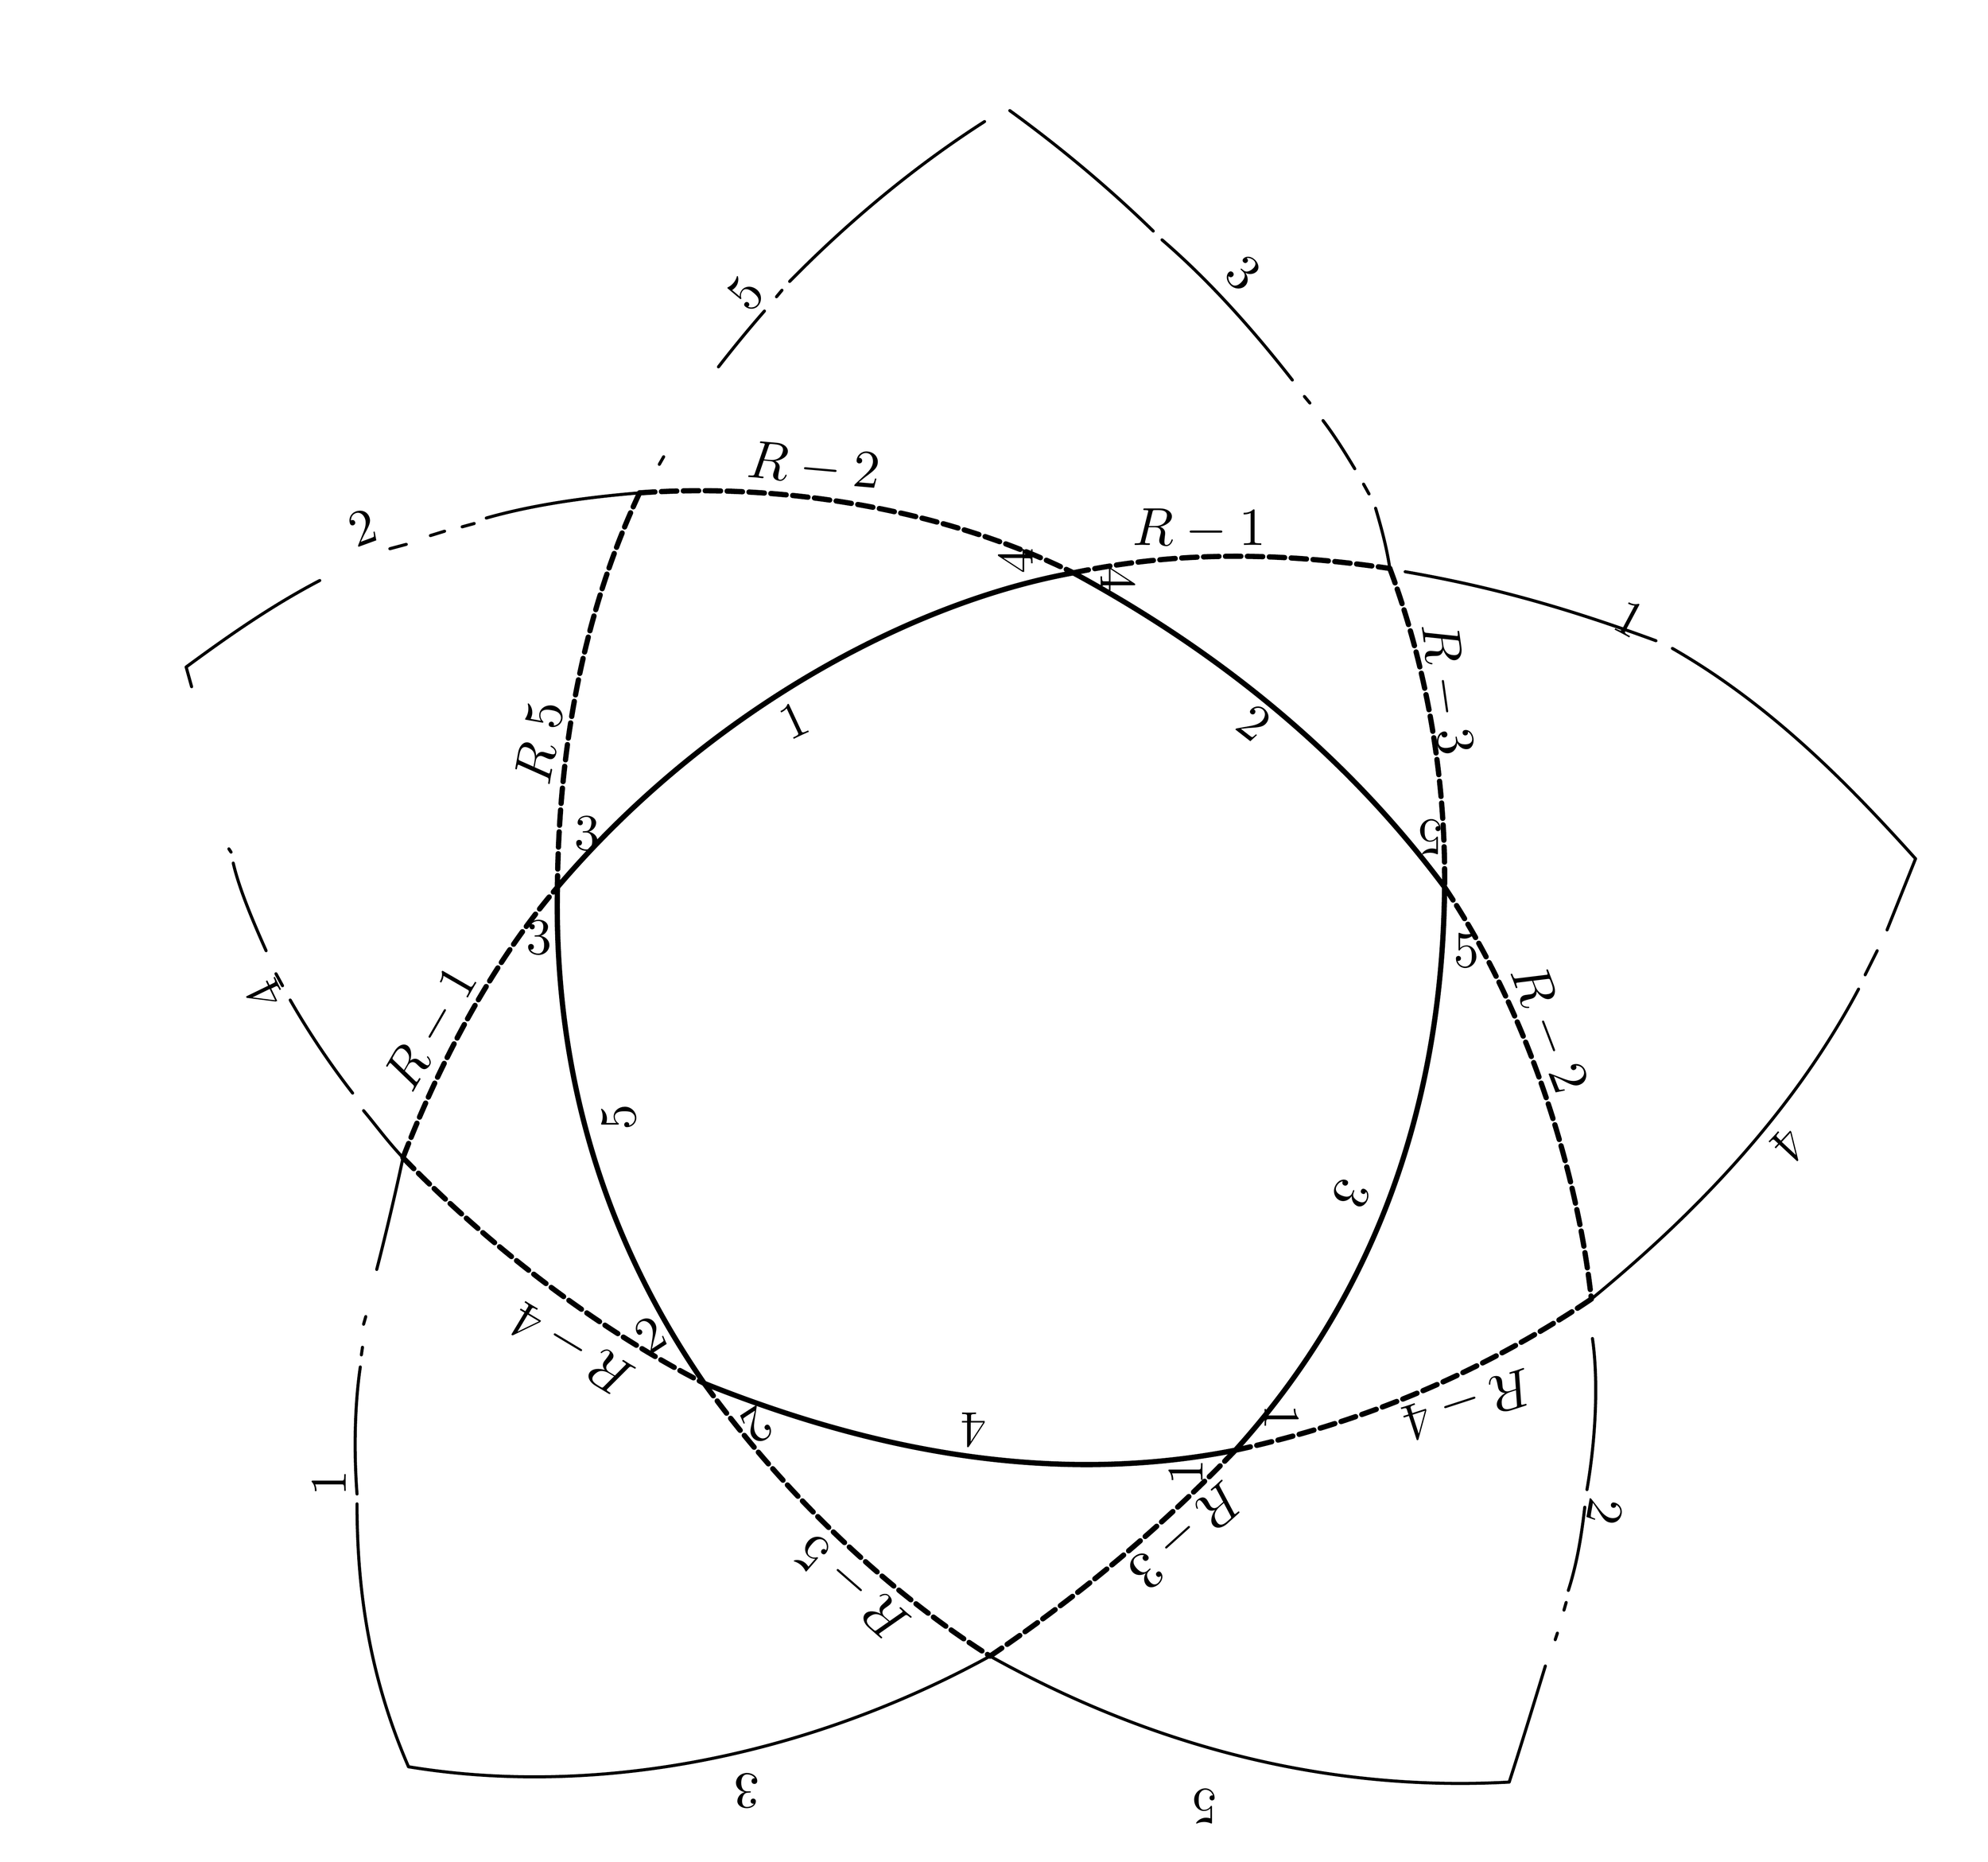
\begin{tikzpicture}[x=1bp,y=-1bp,line cap=round,line join=round]
\path[use as bounding box] (0,0) rectangle (1795,1680);
\begin{pgfinterruptboundingbox}
\draw[line width=4.8bp] (499,800) .. controls (636,639) and (821,540) .. (970,513);
\draw[line width=4.8bp] (970,513) .. controls (1112,590) and (1224,686) .. (1309,800);
\draw[line width=4.8bp] (1309,800) .. controls (1307,1011) and (1238,1181) .. (1118,1314);
\draw[line width=4.8bp] (1118,1314) .. controls (941,1349) and (773,1309) .. (633,1253);
\draw[line width=4.8bp] (633,1253) .. controls (533,1108) and (496,954) .. (499,800);
\draw[line width=4.8bp,dash pattern=on 14bp off 6bp] (358,1047) .. controls (395,951) and (444,864) .. (499,800);
\draw[line width=4.8bp,dash pattern=on 14bp off 6bp] (970,513) .. controls (1075,491) and (1170,496) .. (1259,509);
\draw[line width=4.8bp,dash pattern=on 14bp off 6bp] (574,440) .. controls (714,430) and (861,459) .. (970,513);
\draw[line width=4.8bp,dash pattern=on 14bp off 6bp] (1309,800) .. controls (1381,907) and (1429,1049) .. (1443,1176);
\draw[line width=4.8bp,dash pattern=on 14bp off 6bp] (1259,509) .. controls (1297,611) and (1310,713) .. (1309,800);
\draw[line width=4.8bp,dash pattern=on 14bp off 6bp] (1118,1314) .. controls (1044,1391) and (969,1451) .. (894,1502);
\draw[line width=4.8bp,dash pattern=on 14bp off 6bp] (358,1047) .. controls (442,1133) and (539,1205) .. (633,1253);
\draw[line width=4.8bp,dash pattern=on 14bp off 6bp] (1118,1314) .. controls (1243,1287) and (1351,1238) .. (1443,1176);
\draw[line width=4.8bp,dash pattern=on 14bp off 6bp] (574,440) .. controls (520,555) and (500,681) .. (499,800);
\draw[line width=4.8bp,dash pattern=on 14bp off 6bp] (633,1253) .. controls (712,1362) and (807,1447) .. (894,1502);
\draw[line width=2.8bp] (160,599) .. controls (198,571) and (238,543) .. (282,520);
\draw[line width=2.8bp] (346,491) -- (361,487);
\draw[line width=2.8bp] (383,479) -- (396,475);
\draw[line width=2.8bp] (412,471) -- (423,468);
\draw[line width=2.8bp] (434,463) .. controls (476,451) and (525,444) .. (574,440);
\draw[line width=2.8bp] (646,325) .. controls (660,307) and (674,290) .. (688,274);
\draw[line width=2.8bp] (699,261) -- (704,255);
\draw[line width=2.8bp] (711,247) .. controls (765,192) and (825,142) .. (889,101);
\draw[line width=2.8bp] (912,91) .. controls (959,125) and (1004,163) .. (1043,201);
\draw[line width=2.8bp] (1051,209) .. controls (1094,246) and (1134,291) .. (1170,337);
\draw[line width=2.8bp] (1181,352) -- (1186,358);
\draw[line width=2.8bp] (1198,374) .. controls (1208,387) and (1218,403) .. (1227,418);
\draw[line width=2.8bp] (1235,432) -- (1240,441);
\draw[line width=2.8bp] (1246,454) .. controls (1251,471) and (1256,489) .. (1259,509);
\draw[line width=2.8bp] (1273,512) .. controls (1354,526) and (1423,546) .. (1502,575);
\draw[line width=2.8bp] (1517,582) .. controls (1606,633) and (1676,704) .. (1739,774);
\draw[line width=2.8bp] (1739,774) -- (1713,839);
\draw[line width=2.8bp] (1704,858) -- (1693,880);
\draw[line width=2.8bp] (1687,893) .. controls (1629,1002) and (1543,1094) .. (1443,1176);
\draw[line width=2.8bp] (1444,1212) .. controls (1449,1246) and (1448,1298) .. (1439,1350);
\draw[line width=2.8bp] (1437,1366) .. controls (1434,1392) and (1430,1417) .. (1422,1442);
\draw[line width=2.8bp] (1420,1453) -- (1418,1460);
\draw[line width=2.8bp] (1412,1481) -- (1410,1487);
\draw[line width=2.8bp] (1401,1511) .. controls (1390,1547) and (1379,1583) .. (1368,1617);
\draw[line width=2.8bp] (1368,1617) .. controls (1203,1626) and (1043,1585) .. (894,1502);
\draw[line width=2.8bp] (894,1502) .. controls (732,1591) and (539,1632) .. (363,1603);
\draw[line width=2.8bp] (363,1603) .. controls (331,1529) and (316,1453) .. (316,1363);
\draw[line width=2.8bp] (316,1354) .. controls (313,1314) and (314,1272) .. (319,1238);
\draw[line width=2.8bp] (320,1227) -- (321,1220);
\draw[line width=2.8bp] (322,1199) -- (324,1192);
\draw[line width=2.8bp] (334,1149) .. controls (342,1118) and (351,1080) .. (358,1047);
\draw[line width=2.8bp] (358,1047) .. controls (343,1031) and (333,1017) .. (322,1004);
\draw[line width=2.8bp] (312,988) .. controls (291,961) and (271,931) .. (255,903);
\draw[line width=2.8bp] (248,890) -- (242,879);
\draw[line width=2.8bp] (233,858) .. controls (220,829) and (208,800) .. (203,778);
\draw[line width=2.8bp] (201,768) -- (199,765);
\draw[line width=2.8bp] (160,599) -- (165,617);
\draw[line width=2.8bp] (592,414) -- (596,407);
\node[inner sep=0pt,outer sep=0pt,rotate=25] at (715,648) {\scalebox{4.7}{\ensuremath{1}}};
\node[inner sep=0pt,outer sep=0pt,rotate=-38] at (1135,650) {\scalebox{4.7}{\ensuremath{2}}};
\node[inner sep=0pt,outer sep=0pt,rotate=-112] at (1224,1080) {\scalebox{4.7}{\ensuremath{3}}};
\node[inner sep=0pt,outer sep=0pt,rotate=180] at (879,1295) {\scalebox{4.7}{\ensuremath{4}}};
\node[inner sep=0pt,outer sep=0pt,rotate=90] at (555,1010) {\scalebox{4.7}{\ensuremath{5}}};
\node[inner sep=0pt,outer sep=0pt,rotate=20] at (321,472) {\scalebox{4.7}{\ensuremath{2}}};
\node[inner sep=0pt,outer sep=0pt,rotate=50] at (671,258) {\scalebox{4.7}{\ensuremath{5}}};
\node[inner sep=0pt,outer sep=0pt,rotate=-43] at (1125,239) {\scalebox{4.7}{\ensuremath{3}}};
\node[inner sep=0pt,outer sep=0pt,rotate=-28] at (1478,555) {\scalebox{4.7}{\ensuremath{1}}};
\node[inner sep=0pt,outer sep=0pt,rotate=-133] at (1623,1035) {\scalebox{4.7}{\ensuremath{4}}};
\node[inner sep=0pt,outer sep=0pt,rotate=-100] at (1455,1370) {\scalebox{4.7}{\ensuremath{2}}};
\node[inner sep=0pt,outer sep=0pt,rotate=180] at (1090,1639) {\scalebox{4.7}{\ensuremath{5}}};
\node[inner sep=0pt,outer sep=0pt,rotate=180] at (672,1625) {\scalebox{4.7}{\ensuremath{3}}};
\node[inner sep=0pt,outer sep=0pt,rotate=90] at (291,1344) {\scalebox{4.7}{\ensuremath{1}}};
\node[inner sep=0pt,outer sep=0pt,rotate=116] at (232,898) {\scalebox{4.7}{\ensuremath{4}}};
\node[inner sep=0pt,outer sep=0pt,rotate=-5] at (733,416) {\scalebox{4.9}{\ensuremath{R-2}}};
\node[inner sep=0pt,outer sep=0pt,rotate=0] at (1085,473) {\scalebox{4.9}{\ensuremath{R-1}}};
\node[inner sep=0pt,outer sep=0pt,rotate=-82] at (1311,619) {\scalebox{4.9}{\ensuremath{R-3}}};
\node[inner sep=0pt,outer sep=0pt,rotate=-69] at (1404,929) {\scalebox{4.9}{\ensuremath{R-2}}};
\node[inner sep=0pt,outer sep=0pt,rotate=198] at (1330,1271) {\scalebox{4.9}{\ensuremath{R-4}}};
\node[inner sep=0pt,outer sep=0pt,rotate=222] at (1072,1391) {\scalebox{4.9}{\ensuremath{R-3}}};
\node[inner sep=0pt,outer sep=0pt,rotate=139] at (769,1439) {\scalebox{4.9}{\ensuremath{R-5}}};
\node[inner sep=0pt,outer sep=0pt,rotate=149] at (513,1221) {\scalebox{4.9}{\ensuremath{R-4}}};
\node[inner sep=0pt,outer sep=0pt,rotate=60] at (384,929) {\scalebox{4.9}{\ensuremath{R-1}}};
\node[inner sep=0pt,outer sep=0pt,rotate=80] at (482,668) {\scalebox{4.9}{\ensuremath{R\;5}}};
\node[inner sep=0pt,outer sep=0pt,rotate=90] at (918,502) {\scalebox{4.7}{\ensuremath{4}}};
\node[inner sep=0pt,outer sep=0pt,rotate=-90] at (1010,519) {\scalebox{4.7}{\ensuremath{4}}};
\node[inner sep=0pt,outer sep=0pt,rotate=180] at (1296,754) {\scalebox{4.7}{\ensuremath{5}}};
\node[inner sep=0pt,outer sep=0pt,rotate=0] at (1329,858) {\scalebox{4.7}{\ensuremath{5}}};
\node[inner sep=0pt,outer sep=0pt,rotate=-90] at (1160,1284) {\scalebox{4.7}{\ensuremath{1}}};
\node[inner sep=0pt,outer sep=0pt,rotate=90] at (1073,1334) {\scalebox{4.7}{\ensuremath{1}}};
\node[inner sep=0pt,outer sep=0pt,rotate=33] at (584,1209) {\scalebox{4.7}{\ensuremath{2}}};
\node[inner sep=0pt,outer sep=0pt,rotate=-147] at (681,1291) {\scalebox{4.7}{\ensuremath{2}}};
\node[inner sep=0pt,outer sep=0pt,rotate=0] at (526,751) {\scalebox{4.7}{\ensuremath{3}}};
\node[inner sep=0pt,outer sep=0pt,rotate=0] at (482,846) {\scalebox{4.7}{\ensuremath{3}}};
\end{pgfinterruptboundingbox}
\end{tikzpicture}
